\documentclass[xcolor=svgnames, aspectratio=169]{beamer}
% \usepackage{pgfpages}
\setbeameroption{
  % show notes
  % show notes on second screen=right  % requires pgfpages
  % show only notes
  hide notes
}

\setbeamertemplate{note page}{
  \vspace{1cm}\hspace{1.05\textwidth}
  \vspace{-2.5cm}
  \insertslideintonotes{.2}
  \footnotesize
  \pagecolor{white}
  \insertnote
}

% --- THEME ---
\usetheme[progressbar=frametitle]{metropolis}
\setbeamertemplate{frame numbering}[counter]  % none, counter, fraction

\useoutertheme{metropolis}
\useinnertheme{metropolis}
\usefonttheme{metropolis}
\usecolortheme{spruce}  % spruce, metropolis, dove, crane, beaver, seagull
\setbeamercolor{background canvas}{bg=white}
\definecolor{mygreen}{rgb}{.125,.5,.25}
\usecolortheme[named=mygreen]{structure}
\usefonttheme[onlymath]{serif}

% --- HACKS ---
% Hide numbers on standout slides.
\setbeamertemplate{frame numbering}{
    \ifbool{metropolis@standout}{}{
        \insertframenumber
    }
}
% Avoid font-warning with itemize bullets.
\renewcommand\textbullet{\ensuremath{\bullet}}

\makeatletter
\newcommand{\srcfive}{\@setfontsize{\srcfive}{5pt}{5pt}}
\newcommand{\srcfivefive}{\@setfontsize{\srcfivefive}{5.5pt}{5.5pt}}
\newcommand{\srcsix}{\@setfontsize{\srcsix}{6pt}{6pt}}
\newcommand{\srcsixfive}{\@setfontsize{\srcsixfive}{6.5pt}{6.5pt}}
\newcommand{\srcseven}{\@setfontsize{\srcseven}{7pt}{7pt}}
\makeatother

% --- PACKAGES ---
\usepackage[UKenglish]{babel}
\usepackage[utf8]{inputenc}
\usepackage{lmodern}
\usepackage[T1]{fontenc}

\usepackage{appendixnumberbeamer}
\usepackage{upquote}
\usetikzlibrary{positioning}
\usepackage{minted}
\usepackage{multicol}

% --- SETTINGS ---
\graphicspath{{./figures/}}
\setlength{\fboxsep}{0pt}

% --- OWN COMMANDS ---
\newcommand{\bdra}{\ensuremath{\boldsymbol \Rightarrow }~}
\newcommand{\dra}{\ensuremath{\Rightarrow }~}

% --- TITLE-STUFF ---
\title{3D CSEM modelling in the frequency and Laplace domains}
\subtitle{One story of success and one of failure}
\date{5th December 2019}
\author{Dieter Werthmüller}
\institute{%
  Thursday Talk -- Applied Geophysics \& Petrophysics\\[1em]%
  \tiny
  \includegraphics[height=1cm]{TU_Delft_logo_RGB}\\
  \color{LightSteelBlue}{%
    Faculty of Civil Engineering and Geosciences > Department of Geoscience \&
    Engineering > Section of Applied Geophysics \& Petrophysics%
  }
}

% --- SLIDES ---
\begin{document}
\metroset{block=fill}  % Fills the block-environment

  \maketitle % -------------------------------------------------------------- %

  \section{The Project} % --------------------------------------------------- %

  \begin{frame}[t]%
    {Geophysical Interpretation with Target-Oriented Joint Inversion Modules}
    \vfill
    \begin{columns}
      \column{0.5\textwidth}
        \centering
        \includegraphics[height=1cm]{GitaroJIM-Logo_300ppi}
      \column{0.5\textwidth}
        \centering
        \includegraphics[height=3cm]{logo_martera}
    \end{columns}
    \vfill
    \begin{columns}
      \column{0.5\textwidth}
        \centering
        \href{https://gitarojim.eu}{GitaroJIM.eu}
      \column{0.5\textwidth}
        \centering
        \href{https://www.martera.eu}{MarTERA.eu}
    \end{columns}
    \centering
    \vfill
    \emph{Project duration: 3 years (June 2018 -- May 2021)}\\[1em]
    % \tiny Funded through Gitaro.JIM, a project of MarTERA as part of Horizon
    % 2020, a funding scheme of the European Research Area.
  \end{frame}

  \begin{frame}[t]%
    {Gitaro.JIM -- Partners}
    \centering
    \hfill
    % GEOMAR Helmholtz Centre for Ocean Research
    \includegraphics[height=1.5cm]{Logo-GEOMAR-300x153}
    % https://www.geomar.de
    \hfill
    % GFZ German Research Centre for Geosciences
    \includegraphics[height=1.5cm]{Logo-GFZ-300x211}
    % https://www.gfz-potsdam.de
    \hfill
    % Delft University of Technology
    \includegraphics[height=1.5cm]{TU_Delft_logo_RGB}
    % https://www.tudelft.nl
    \hfill~\\[1cm]
    \hfill
    % TEEC GmbH
    \includegraphics[height=1.25cm]{Logo-TEEC-207x102}
    % https://teec.de
    \hfill
    % TERRASYS Geophysics GmbH \& Co. KG
    \includegraphics[height=1cm]{Logo-TERRASYS-768x145}
    % http://www.terrasys.de
    \hfill~\\
    \vfill
    Supported by \alert{University of Southampton} and \alert{Equinor}\\[.5em]
    Member of the \alert{Delphi Consortium}
  \end{frame}

  \begin{frame}%
    {Gitaro.JIM -- Objectives}
    \includegraphics[height=9cm]{InversionFramework}
  \end{frame}

  \begin{frame}[t]%
    {Gitaro.JIM -- Data}
    \begin{columns}[t]
      \column{.33\textwidth}
        \centering
        \alert{Methane Hydrates}\\
        Danube Paleo Delta\\
        Black Sea\\[1cm]
        \frame{\includegraphics[width=\columnwidth]{black_sea_map}}
      \column{.33\textwidth}
        \centering
        \alert{Oil \& Gas}\\
        Nordkapp Basin\\
        Barents Sea\\[1cm]
        \frame{\includegraphics[width=\columnwidth]{nordkapp_enhanced_gravity}}
      \column{.33\textwidth}
        \centering
        \alert{Seafloor Massive Sulfides}\\
        Palinuro\\
        Tyrrhenian Sea\\[1cm]
        \frame{\includegraphics[width=\columnwidth]{tyrrhenian_sea_map}}
    \end{columns}
  \end{frame}

  \begin{frame}%
    {Gitaro.JIM -- TU Delft}
    \begin{itemize}\itemsep.6cm
      \item 3D CSEM modelling; frequency domain
      \item Comparison to existing code; frequency domain and time domain
      \item Inversion
      \item Anisotropy
      \item Topopgraphy
    \end{itemize}
  \end{frame}

  \section{The Code} % ------------------------------------------------------ %

  \begin{frame}%
    {Multigrid CSEM code by Mulder et al.}
    \vfill
    \begin{block}{W.A. Mulder, T.B. Jönsthövel, M. Wirianto, E.C. Slob, R.-E.
      Plessix, \ldots}
      \begin{equation}
        -s \sigma \mathbf{\hat{E}} - \nabla \times \mu^{-1} \nabla
        \times \mathbf{\hat{E}} = s\mathbf{\hat{J}}
            \nonumber
      \end{equation}
    \end{block}
    \vfill
    \begin{columns}
      \column{.3\textwidth}
        \begin{itemize}
          \item Matlab/C
          \item Multigrid
          \item Finite Volumes
          \item VTI resistivity
        \end{itemize}
      \column{.5\textwidth}
        \fbox{\includegraphics[width=\linewidth]{gp2006}}
      \end{columns}
  \end{frame}

  \begin{frame}%
    {emg3d  -- Open-source multigrid solver for 3D EM diffusion}
    \vfill
    \begin{columns}
      \column{.5\textwidth}
      \centering
        \includegraphics[width=.8\linewidth]{logo-emg3d}\\
      \column{.5\textwidth}
        \begin{itemize}
          \item Python/Numba
          \item Apache v2.0
          \item \href{https://empymod.github.io}{empymod.github.io}
        \end{itemize}
    \end{columns}
    \vfill
    \begin{columns}
      \column{.8\textwidth}
    \begin{block}{Installation}
      \vspace{0.5em}
      \begin{description}
        \item[conda:] \texttt{conda install -c conda-forge emg3d}
        \item[pip:] \texttt{pip install emg3d}
      \end{description}
      \centering
      \textbf{Requirements:} \texttt{NumPy}, \texttt{SciPy}, \texttt{Numba},
      \texttt{empymod}; \texttt{Python 3.7+}
      \vspace{0.5em}
    \end{block}
  \end{columns}
  \end{frame}

  \begin{frame}[t]%
    {Multigrid method}
    \begin{columns}
      \column{.5\textwidth}
        \centering
        \alert{Matrix-free solver}\\[1em]
      \column{.5\textwidth}
        \centering
        \alert{Restriction and prolongation}\\[1em]
    \end{columns}
    \vspace{1em}
    \begin{columns}
      \column{.5\textwidth}
        \centering

        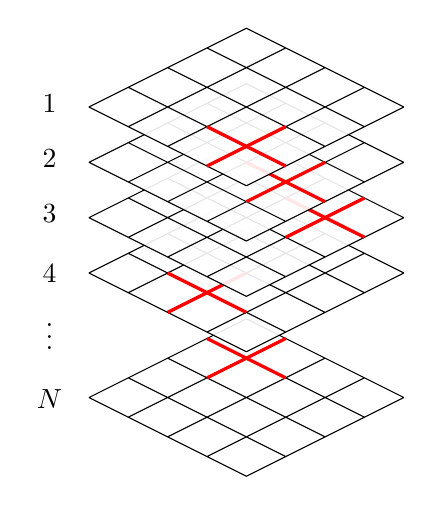
\begin{tikzpicture}[scale=0.5, auto,swap]

          % Nth smoothing step
          \node at (-5, -0.5) {$N$};
          \begin{scope}[
                  yshift=-70,every node/.append style={
                  yslant=0.5,xslant=-1},yslant=0.5,xslant=-1
                  ]
              \fill[white,fill opacity=0.9] (0,0) rectangle (4,4);
              \draw[step=10mm] (0,0) grid (4,4);
              \draw[red, very thick] (3,3) -- (2,3);
              \draw[red, very thick] (3,3) -- (3,2);
              \draw[red, very thick] (3,3) -- (4,3);
              \draw[red, very thick] (3,3) -- (3,4);
          \end{scope}

          % \ldots
          \node at (-5, 1.3) {\vdots};
          \begin{scope}[
              yshift=0,every node/.append style={
                  yslant=0.5,xslant=-1},yslant=0.5,xslant=-1
                          ]
          \end{scope}

          % 4nd smoothing step
          \node at (-5, 2.7) {$4$};
          \begin{scope}[
              yshift=20,every node/.append style={
              yslant=0.5,xslant=-1},yslant=0.5,xslant=-1
                          ]
              \fill[white,fill opacity=0.9] (0,0) rectangle (4,4);
              \draw[step=10mm] (0,0) grid (4,4);
              \draw[red, very thick] (1,2) -- (0,2);
              \draw[red, very thick] (1,2) -- (1,1);
              \draw[red, very thick] (1,2) -- (2,2);
              \draw[red, very thick] (1,2) -- (1,3);
          \end{scope}

          % 3nd smoothing step
          \node at (-5, 4.2) {$3$};
          \begin{scope}[
              yshift=60,every node/.append style={
              yslant=0.5,xslant=-1},yslant=0.5,xslant=-1
                          ]
              \fill[white,fill opacity=0.9] (0,0) rectangle (4,4);
              \draw[step=10mm] (0,0) grid (4,4);
              \draw[red, very thick] (3,1) -- (2,1);
              \draw[red, very thick] (3,1) -- (3,0);
              \draw[red, very thick] (3,1) -- (4,1);
              \draw[red, very thick] (3,1) -- (3,2);
          \end{scope}

          % 2nd smoothing step
          \node at (-5, 5.6) {$2$};
          \begin{scope}[
              yshift=100,every node/.append style={
              yslant=0.5,xslant=-1},yslant=0.5,xslant=-1
                          ]
              \fill[white,fill opacity=0.9] (0,0) rectangle (4,4);
              \draw[step=10mm] (0,0) grid (4,4);
              \draw[red, very thick] (2,1) -- (1,1);
              \draw[red, very thick] (2,1) -- (2,0);
              \draw[red, very thick] (2,1) -- (3,1);
              \draw[red, very thick] (2,1) -- (2,2);
          \end{scope}

          % 1st smoothing step
          \node at (-5, 7) {$1$};
          \begin{scope}[
              yshift=140,every node/.append style={
                  yslant=0.5,xslant=-1},yslant=0.5,xslant=-1
                ]
              \fill[white,fill opacity=0.9] (0,0) rectangle (4,4);
              \draw[step=10mm] (0,0) grid (4,4);
              \draw[red, very thick] (1,1) -- (0,1);
              \draw[red, very thick] (1,1) -- (1,0);
              \draw[red, very thick] (1,1) -- (2,1);
              \draw[red, very thick] (1,1) -- (1,2);

          \end{scope}

        \end{tikzpicture}

      \column{.5\textwidth}
        \centering

        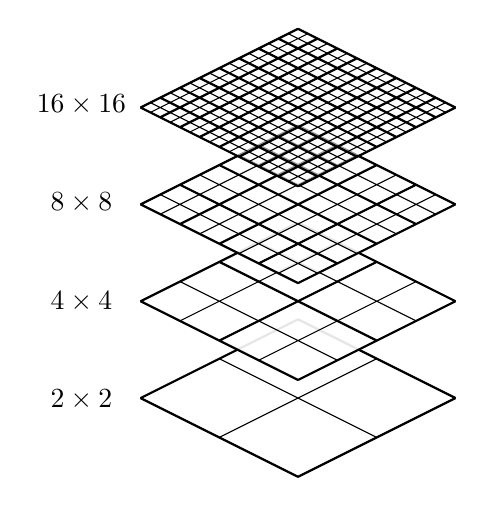
\begin{tikzpicture}[scale=0.5, auto,swap]
          % 2x2 Coarsest grid
          \node at (-5.5, -0.5) {$2\times2$};
          \begin{scope}[
                  yshift=-70,every node/.append style={
                  yslant=0.5,xslant=-1},yslant=0.5,xslant=-1
                  ]
              \fill[white,fill opacity=0.9] (0,0) rectangle (4,4);
              \draw[step=40mm, thick] (0,0) grid (4,4);
              \draw[step=20mm] (0,0) grid (4,4);
          \end{scope}

          % 4x4
          \node at (-5.5, 2) {$4\times4$};
          \begin{scope}[
              yshift=0,every node/.append style={
                  yslant=0.5,xslant=-1},yslant=0.5,xslant=-1
                          ]
              \fill[white,fill opacity=.9] (0,0) rectangle (4,4);
              \draw[step=20mm, thick] (0,0) grid (4,4);
              \draw[step=10mm] (0,0) grid (4,4);
          \end{scope}

          % 8x8
          \node at (-5.5, 4.5) {$8\times8$};
          \begin{scope}[
              yshift=70,every node/.append style={
              yslant=0.5,xslant=-1},yslant=0.5,xslant=-1
                          ]
              \fill[white,fill opacity=.9] (0,0) rectangle (4,4);
              \draw[step=10mm, thick] (0,0) grid (4,4);
              \draw[step=5mm] (0,0) grid (4,4);
          \end{scope}

          % 16x16 Finest grid
          \node at (-5.5, 7) {$16\times16$};
          \begin{scope}[
              yshift=140,every node/.append style={
                  yslant=0.5,xslant=-1},yslant=0.5,xslant=-1
                ]
              \fill[white,fill opacity=0.6] (0,0) rectangle (4,4);
              \draw[step=5mm, thick] (0,0) grid (4,4);
              \draw[step=2.5mm] (0,0) grid (4,4);

          \end{scope}

        \end{tikzpicture}

    \end{columns}

  \end{frame}

  \begin{frame}[t]%
    {Multigrid -- CPU \& RAM}
    \vspace{1em}
    \begin{columns}
      \column{.5\textwidth}
        \centering
        \alert{CPU}\\[1em]
      \column{.5\textwidth}
        \centering
        \alert{RAM}\\[1em]
    \end{columns}
    \vspace{1em}
    \begin{columns}
      \column{.5\textwidth}
        \centering
        \includegraphics[width=\linewidth]{runtime}
      \column{.5\textwidth}
        \centering
        \includegraphics[width=\linewidth]{RAM-Usage}
    \end{columns}
    \centering
    \vspace{.5em}
    Measured on \texttt{texel}, single thread
  \end{frame}

  \section{Frequency Domain} % ---------------------------------------------- %

  % --- Define code examples --- %
  \defverbatim[colored]{\mwecode}{%
    \begin{minted}[fontsize=\srcsixfive]{python}
import emg3d
import discretize

grid = discretize.TensorMesh(
        [[(25, 48)], [(50, 32)], [(30, 32)]],
        x0='CCC')

model = emg3d.utils.Model(
        grid, res_x=1.5, res_y=1.8, res_z=3.3)

sfield = emg3d.utils.get_source_field(
        grid, src=[0, 0, 0, 0, 0], freq=10)

efield = emg3d.solver.solver(
        grid, model, sfield, verb=3)
    \end{minted}
  }

  \defverbatim[colored]{\mweplot}{%
    \begin{minted}[fontsize=\srcsixfive]{python}
grid.plot_3d_slicer(
      efield.fx.ravel('F'), view='abs', vType='Ex',
      pcolorOpts={'norm': LogNorm()})
    \end{minted}
  }

  \defverbatim{\mwelog}{%
    \begin{minted}[fontsize=\srcsix]{text}
:: emg3d START :: 10:28:27 :: v0.9.1

   MG-cycle       : 'F'                 sslsolver : False
   semicoarsening : False [0]           tol       : 1e-06
   linerelaxation : False [0]           maxit     : 50
   nu_{i,1,c,2}   : 0, 2, 1, 2          verb      : 3
   Original grid  :  48 x  32 x  32     => 49,152 cells
   Coarsest grid  :   3 x   2 x   2     => 12 cells
   Coarsest level :   4 ;   4 ;   4   

   [hh:mm:ss]  rel. error                  [abs. error, last/prev]   l s

       h_
      2h_ \                  /
      4h_  \          /\    / 
      8h_   \    /\  /  \  /  
     16h_    \/\/  \/    \/   

   [10:28:27]   2.623e-02  after   1 F-cycles   [1.464e-06, 0.026]   0 0
   [10:28:28]   2.253e-03  after   2 F-cycles   [1.258e-07, 0.086]   0 0
   [10:28:28]   3.051e-04  after   3 F-cycles   [1.704e-08, 0.135]   0 0
   [10:28:29]   5.501e-05  after   4 F-cycles   [3.071e-09, 0.180]   0 0
   [10:28:29]   1.170e-05  after   5 F-cycles   [6.532e-10, 0.213]   0 0
   [10:28:30]   2.745e-06  after   6 F-cycles   [1.533e-10, 0.235]   0 0
   [10:28:30]   6.874e-07  after   7 F-cycles   [3.838e-11, 0.250]   0 0

   > CONVERGED
   > MG cycles        : 7
   > Final rel. error : 6.874e-07

:: emg3d END   :: 10:28:30 :: runtime = 0:00:03
    \end{minted}
  }

  \begin{frame}[t]%
    {emg3d -- Minimal Example}
    \begin{columns}
      \column{0.45\textwidth}
        \begin{minipage}{.45\textwidth}
          \only<2>{\vspace{-1.5cm}}
          \mwecode
          \uncover<3>{\mweplot}
          \vfill
        \end{minipage}
      \column{0.55\textwidth}
        \only<2>{
          \begin{minipage}{.55\textwidth}
            \vspace{-.5cm}
            \mwelog
          \end{minipage}
        }
        \only<3>{
          \includegraphics[width=\textwidth]{minimal-example}
        }
    \end{columns}
  \end{frame}

  \defverbatim{\seglog}{%
    \begin{minted}[fontsize=\srcfive]{text}
:: emg3d START :: 10:36:50 :: v0.9.1

   MG-cycle       : 'F'                 sslsolver : 'bicgstab'
   semicoarsening : False [0]           tol       : 1e-06
   linerelaxation : False [0]           maxit     : 50 (1)
   nu_{i,1,c,2}   : 0, 2, 1, 2          verb      : 3
   Original grid  : 128 x 128 x 128     => 2,097,152 cells
   Coarsest grid  :   2 x   2 x   2     => 8 cells
   Coarsest level :   6 ;   6 ;   6   

   [hh:mm:ss]  rel. error            solver              MG          l s

   [10:37:03]   1.591e-01  after                       1 F-cycles    0 0
   [10:37:15]   3.299e-02  after                       2 F-cycles    0 0
   [10:37:16]   2.291e-02  after   1 bicgstab-cycles
   [10:37:26]   6.756e-03  after                       3 F-cycles    0 0
   [10:37:37]   1.035e-03  after                       4 F-cycles    0 0
   [10:37:38]   8.113e-04  after   2 bicgstab-cycles
   [10:37:51]   3.055e-04  after                       5 F-cycles    0 0
   [10:38:01]   6.347e-05  after                       6 F-cycles    0 0
   [10:38:02]   4.581e-05  after   3 bicgstab-cycles
   [10:38:14]   1.753e-05  after                       7 F-cycles    0 0
   [10:38:27]   4.368e-06  after                       8 F-cycles    0 0
   [10:38:28]   3.969e-06  after   4 bicgstab-cycles
   [10:38:43]   2.619e-06  after                       9 F-cycles    0 0
   [10:38:55]   1.626e-06  after                      10 F-cycles    0 0
   [10:38:56]   1.127e-06  after   5 bicgstab-cycles
   [10:39:07]   8.366e-07  after                      11 F-cycles    0 0
   [10:39:08]   7.448e-07  after   6 bicgstab-cycles

   > CONVERGED
   > Solver steps     : 6
   > MG prec. steps   : 11
   > Final rel. error : 7.448e-07

:: emg3d END   :: 10:39:08 :: runtime = 0:02:18
    \end{minted}
  }

  \begin{frame}%
    {emg3d -- SEG-EAGE salt model$\,^\dagger$}
    \only<1>{\vspace{1em}}
    \begin{columns}
      \column{.5\textwidth}
        \centering
        \only<1>{
          $\approx$ 96 million cells {\small (only model)}\\
          {\small $(20\mathrm{m}\times20\mathrm{m}\times20\mathrm{m})$}
          \includegraphics[width=\textwidth]{seg-salt-fine}
        }
        \only<2>{
          \includegraphics[width=\textwidth]{seg-salt-result}
        }
      \column{.5\textwidth}
        \centering
        \only<1>{
          $\approx$ 2.1 million cells {\small (+ air \& boundary)}\\
          {\small (x/y: $55-182\,\mathrm{m}$; z: $20-517\,\mathrm{m}$)}
          \includegraphics[width=\textwidth]{seg-salt-coarse}
        }
        \only<2>{
          \begin{minipage}{.5\textwidth}
            \seglog
          \end{minipage}
        }
    \end{columns}
    \only<1>{\tiny $^\dagger$ SEG-EAGE salt model: Aminzadeh et al. (1997);
      Velocity-to-resistivity conversion: Mulder (2007).}

  \end{frame}

  \section{Time Domain} % --------------------------------------------------- %

  \begin{frame}
    {Plessix et al., 2007 \& Mulder et al., 2008}
    \begin{columns}[t]
      \column{.5\textwidth}
      \alert{Automatic gridding}
      \begin{equation}
        \delta = \sqrt{\frac{2}{\omega\mu\sigma}} \approx
        \quad 503.3/\sqrt{f\sigma} \, ,
        \nonumber
      \end{equation}
      \begin{itemize}
        \item Minimum cell width
          $\mathrm{func}(\delta_\mathrm{s}, L_\mathrm{s}, \mathrm{pps}$)
        \item Domains:
          $\mathrm{pps}\cdot\delta_\mathrm{ave}$
          \begin{itemize}
            \item Core domain: $\mathrm{pps}\approx 4-8\ (3-8)$
            \item Boundary domain: $\mathrm{pps}\approx 4\ (5)$
            \item Air (upwards $z$): 50\,km
          \end{itemize}
        \item Mapping by volume averaging
        \item \textbf{Find optimal $\boldsymbol{\alpha}$ for a fixed \#cells}
      \end{itemize}
      \column{.5\textwidth}
      \alert{Adaptive frequency selection}
      \begin{itemize}
        \item Start: $f_\mathrm{min}-f_\mathrm{max}$, 1/dec
        \item Add more frequencies left and right of $f_i$ if
          $|E_\mathrm{int}(f_i)-E_\mathrm{calc}(f_i)|>\mathrm{tol}$
      \end{itemize}
      \vspace{1em}
      \centering
      \includegraphics[width=.8\textwidth]{mulder08fig1}
    \end{columns}
  \end{frame}

  \begin{frame}%
    {Changes to existing schemes}
    \begin{columns}
      \column{.5\textwidth}
      \alert{(a) code}
      \begin{itemize}
        \item Flexible \#cell, in each direction
        \item Mult. with any low prime, $\{2,3,5\}\cdot2^n$\\
          e.g., ${\mathbf{64},  80,  96, \mathbf{128}, 160, 192, \mathbf{256}}$
      \end{itemize}
      \vspace{2em}
      \alert{(c) $f$-selection and Fourier transform}
      \begin{itemize}
        \item Regular spacing (log-scale)
        \item A logarithmic Fourier transform
          \begin{itemize}
            \item Digital Linear Filters (DLF)$^\dagger$
            \item FFTLog $^\ddagger$
          \end{itemize}
      \end{itemize}
      \column{.5\textwidth}
      \alert{(b) automatic gridding}
      \begin{itemize}
        \item Define core domain
        \item \textbf{Search for minimal number of cells}
        \begin{itemize}
          \item $\alpha$-range for core domain
          \item $\alpha$-range for boundary domain
        \end{itemize}
        \item Careful regarding the air layer
      \end{itemize}
    \end{columns}
    {\tiny $^\dagger$ Ghosh (1970); $^\ddagger$ Hamilton (2000)}
  \end{frame}

  \begin{frame}%
    {Mulder et al., 2008; Figures 2-4; homogeneous fullspace}
    \begin{itemize}
      \item 26 frequencies, 0.01\,Hz$-$100\,Hz
      \item Runtime: 3h\,47\,min\,12\,s
      \item The peak value has an error of about 1\,\%
    \end{itemize}
    \begin{columns}[t]
      \column{1.15\textwidth}
        \centering
        \includegraphics[width=.32\textwidth]{mulder08fig2}
        \includegraphics[width=.32\textwidth]{mulder08fig3}
        \includegraphics[width=.32\textwidth]{mulder08fig4}
    \end{columns}
  \end{frame}

  \begin{frame}%
    {Our result, 2019}
    \begin{itemize}
      \item 14 frequencies, 0.05\,Hz$-$20\,Hz
      \item Runtime: 1\,min\,40\,s
      \item The peak value has an error of about 0.01\,\%
    \end{itemize}
    \begin{columns}[t]
      \column{1.1\textwidth}
        \centering
        \includegraphics[width=\textwidth]{fullspace-comp}
    \end{columns}
  \end{frame}

  \defverbatim{\timelog}{%
    \begin{minted}[fontsize=\srcsix]{text}
              **** TOTAL RUNTIME :: 0:01:40 ****

 20.036 Hz:  4/1 it;   4 s;  a: 1.00 / 1.18;  n: 80 x 24 x 24;  d: 20 /  138
 12.642 Hz:  7/1 it;   6 s;  a: 1.00 / 1.22;  n: 80 x 24 x 24;  d: 20 /  192
  7.977 Hz:  7/1 it;   6 s;  a: 1.00 / 1.25;  n: 80 x 24 x 24;  d: 20 /  265
  5.033 Hz:  7/1 it;   6 s;  a: 1.00 / 1.29;  n: 80 x 24 x 24;  d: 20 /  364
  3.176 Hz:  7/1 it;   5 s;  a: 1.00 / 1.30;  n: 80 x 24 x 24;  d: 24 /  422
  2.004 Hz:  7/1 it;   4 s;  a: 1.00 / 1.30;  n: 64 x 24 x 24;  d: 30 /  531
  1.264 Hz:  7/1 it;   4 s;  a: 1.00 / 1.30;  n: 64 x 24 x 24;  d: 37 /  669
  0.798 Hz:  7/1 it;   7 s;  a: 1.00 / 1.20;  n: 64 x 24 x 24;  d: 40 /  616
  0.503 Hz:  7/1 it;   7 s;  a: 1.00 / 1.23;  n: 64 x 24 x 24;  d: 40 /  893
  0.318 Hz:  7/1 it;   9 s;  a: 1.00 / 1.25;  n: 64 x 24 x 24;  d: 40 / 1137
  0.200 Hz:  7/1 it;   7 s;  a: 1.00 / 1.28;  n: 64 x 24 x 24;  d: 40 / 1623
  0.126 Hz:  7/1 it;   7 s;  a: 1.00 / 1.30;  n: 64 x 24 x 24;  d: 40 / 2047
  0.080 Hz:  7/1 it;  13 s;  a: 1.00 / 1.25;  n: 64 x 32 x 32;  d: 40 / 2220
  0.050 Hz:  7/1 it;  12 s;  a: 1.00 / 1.27;  n: 64 x 32 x 32;  d: 40 / 2955
    \end{minted}
  }

  \begin{frame}%
    {Analysis -- Overview and gridding}
    Main reasons for speed-up of 136x:
    \begin{itemize}
      \item ++ Automatic gridding; transform; cell sizes
      \item + Computers faster in the last 11 years
      \item $\approx$ Different implementation (Matlab/C vs Python/Numba)
    \end{itemize}

    \begin{columns}
      \column{.6\textwidth}
        \begin{minipage}{\textwidth}
          \timelog
        \end{minipage}
    \end{columns}
  \end{frame}

  \begin{frame}%
    {Analysis -- Frequency Calculation}
    \centering
      \includegraphics[width=.8\textwidth]{fullspace-freq}
  \end{frame}


  \section{Laplace Domain} % ------------------------------------------------ %

  \begin{frame}%
    {Laplace $s$: $ -s \sigma \mathbf{\hat{E}} - \nabla \times \mu^{-1} \nabla
        \times \mathbf{\hat{E}} = s\mathbf{\hat{J}}
        \quad \Rightarrow \quad s =
        \mathrm{i}\omega = 2\mathrm{i}\pi f
        \text{ or } s
      $}
      \includegraphics[width=.85\textwidth]{motivationcomparison}
  \end{frame}

  \begin{frame}%
    {Laplace -- faster calculation, faster convergence}
    \vfill
    \begin{columns}[t]
      \column{.5\textwidth}
        \alert{Frequency domain}
        \begin{itemize}
          \item 9--10\,s per F-cycle
          \item 5 BiCGSTAB cycles; 9 MG cycles
          \item 1\,min 32\,s
        \end{itemize}
      \column{.5\textwidth}
        \alert{Laplace domain}
        \begin{itemize}
          \item 7--8\,s per F-cycle
          \item 4 BiCGSTAB cycles; 8 MG cycles
          \item 1\,min 2\,s \dra 1/3 faster!
        \end{itemize}
    \end{columns}
    \vspace{1em}

    \begin{columns}[t]
      \column{.5\textwidth}
        \fbox{\includegraphics[trim=0 0 0 11.7cm, clip, width=.9\textwidth]%
                              {runtime-frequency}}
      \column{.5\textwidth}
        \fbox{\includegraphics[trim=0 0 0 11.7cm, clip, width=.9\textwidth]%
                              {runtime-Laplace}}
    \end{columns}
  \end{frame}

  \begin{frame}%
    {DLF Laplace-to-time}
    \vspace{-1em}
    \begin{equation}
      F(r) = \int^\infty_0 f(l)K(l r)\mathrm{d}l
      \qquad \underrightarrow{r = e^x, l = e^{-y}} \qquad
      F(r) \approx \sum^N_{n=1} \frac{f(b_n/r) h_n}{r}
      \nonumber
    \end{equation}
    \centering
      \includegraphics[width=.8\textwidth]{filter-space}

    {\tiny $^\dagger$ DLF-method: Ghosh (1970); Used tool: Werthmüller et al.
    (2019)}

  \end{frame}

  \begin{frame}%
    {Test using empymod }
    \centering
      \includegraphics[width=.7\textwidth]{s2tempymod}
  \end{frame}

  \begin{frame}%
    {Laplace -- It doesn't work}
    \centering
      \includegraphics[width=.8\textwidth]{s-t_time}
  \end{frame}

  \section{Summary} % ------------------------------------------------------- %

  \begin{frame}%
    {Summary}
    \centering
    \begin{columns}
      \column{.45\textwidth}
        \begin{itemize}\itemsep.3cm
          \item \textbf{emg3d}
          \item \textbf{Frequency-domain} calculation
          \item \textbf{Laplace-domain} calculation
        \end{itemize}
      \column{.55\textwidth}
        \begin{itemize}\itemsep.3cm
          \item \textbf{Time-domain} calculation
            \begin{itemize}
              \item Significant speed-up using the $f$-domain
              \item Not working using the $s$-domain
            \end{itemize}
        \end{itemize}
    \end{columns}
    \vfill
    \alert{Slides:}
    \href{https://github.com/empymod/presentations/tree/master/ThursdayTalk2019}%
    {\textbf{github.com/empymod} \dra presentations \dra ThursdayTalk2019}
  \end{frame}

  \begin{frame}%
    {References}
    \begin{columns}
      \column{1.1\textwidth}
    \setlength{\columnseprule}{0.4pt}
    % \setlength{\columnsep}{3em}
    \begin{multicols}{2}
    \tiny
    \begin{description}[2cm]
      %
      \item[Aminzadeh, F., Brac, J., and Kunz, T., 1997,] {\bfseries SEG/EAGE
        3-D Salt and Overthrust Models:} SEG, Tulsa, Oklahoma;
        \href{https://wiki.seg.org/wiki/SEG/EAGE_Salt_and_Overthrust_Models}%
        {wiki.seg.org/wiki/SEG/EAGE\_Salt\_and\_Overthrust\_Models}.
      %
      \item[Ghosh, D. P.,  1970,] {\bfseries The application of linear filter
        theory to the direct interpretation of geoelectrical resistivity
        measurements:} Ph.D. Thesis, TU Delft;
        \href{http://resolver.tudelft.nl/uuid:88a568bb-ebee-4d7b-92df-6639b42da2b2}%
        {uuid:~88a568bb-ebee-4d7b-92df-6639b42da2b2}.
      %
      \item[Hamilton, A. J. S., 2000,] {\bfseries Uncorrelated modes of the
        non-linear power spectrum:} Monthly Notices of the Royal Astronomical
        Society, 312, pages 257--284;
        \href{https://doi.org/10.1046/j.1365-8711.2000.03071.x}%
        {doi:~10.1046/j.1365-8711.2000.03071.x}.
      %
      \item[Jönsthövel, T. B., C. W. Oosterlee, and W. A. Mulder, 2006,]
        {\bfseries Improving multigrid for 3-D electro-magnetic diffusion on
        stretched grids:} European Conference on Computational Fluid Dynamics;
        \href{http://resolver.tudelft.nl/uuid:df65da5c-e43f-47ab-b80d-2f8ee7f35464}
        {UUID:~df65da5c-e43f-47ab-b80d-2f8ee7f35464}.
      %
      \item[Mulder, W. A., 2006,] {\bfseries A multigrid solver for {3D}
        electromagnetic diffusion:} Geophysical Prospecting, 54, 633--649;
        \href{https://doi.org/10.1111/j.1365-2478.2006.00558.x}%
        {doi:~10.1111/j.1365-2478.2006.00558.x}.
      %
      \item[Mulder, W. A., 2007,] {\bfseries A robust solver for CSEM modelling
        on stretched grids:} EAGE Technical Program Expanded Abstracts, D036;
        \href{https://doi.org/10.3997/2214-4609.201401567}%
        {doi:~10.3997/2214-4609.201401567}.
      %
      \item[Mulder, W. A., M. Wirianto, and E. Slob, 2008,] {\bfseries
        Time-domain modeling of electromagnetic diffusion with a
        frequency-domain code:} Geophysics, 73, F1--F8;
        \href{https://doi.org/10.1190/1.2799093}{doi:~10.1190/1.2799093}.
      %
      \item[Plessix, R.-E., M. Darnet, and W. A. Mulder, 2007,] {\bfseries An
        approach for 3D multisource, multifrequency CSEM modeling:} Geophysics,
        72, SM177--SM184;
        \href{https://doi.org/10.1190/1.2744234}{doi:~10.1190/1.2744234}.
      %
      \item[Werthmüller, D., 2017,] {\bfseries An open-source full 3D
          electromagnetic modeler for 1D VTI media in Python: empymod:}
          Geophysics, 82(6), WB9--WB19;
          \href{https://doi.org/10.1190/geo2016-0626.1}%
          {doi:~10.1190/geo2016-0626.1}.
      %
      \item[Werthmüller, D., K. Key, and E. C. Slob, 2019,] {\bfseries A tool
          for designing digital filters for the Hankel and Fourier transforms
          in potential, diffusive, and wavefield modeling:} Geophysics, 84(2),
          F47--F56; \href{https://doi.org/10.1190/geo2018-0069.1}%
          {doi:~10.1190/geo2018-0069.1}.
      %
      \item[Werthmüller, D., W. A. Mulder, and E. C. Slob, 2019,] {\bfseries
        emg3d: A multigrid solver for 3D electromagnetic diffusion:} Journal of
        Open Source Software, 4(39), 1463;
        \href{https://doi.org/10.21105/joss.01463}{doi:~10.21105/joss.01463}.
      %
    \end{description}
  \end{multicols}
  \end{columns}
  \end{frame}

  \begin{frame}%
    {Swung (software underground)}
    \centering
    \fbox{\includegraphics[width=.55\textwidth]{swung}}\\
    \vfill
    Hackathon EAGE 2020: 06/07 June 2020 (\#amstel-hack-2020)
  \end{frame}

  \appendix % ------- finished, stop numbering ------------------------------ %

  \maketitle % ------ title again ------------------------------------------- %

  \section{Appendix} % ------------------------------------------------------ %

  \begin{frame}[t]%
    {emg3d -- CI workflow}
    \begin{columns}[t]
      \column{0.45\textwidth}
      \begin{itemize}
        \item Commit to GitHub
        \item Travis CI - run all tests
          \begin{itemize}
            \item Report to coveralls
            \item Check all hyperlinks
            \item Deploy to PyPi (\emph{if tag})
            \item Deploy to conda-forge (\emph{if tag})
          \end{itemize}
        \item Codacy
        \item ReadTheDocs and Gallery
        \item Zenodo (\emph{if tag})
        \item Benchmarks (\texttt{asv}, \emph{manual})
      \end{itemize}
      \column{0.55\textwidth}
        \vspace{.5cm}
        \only<1>{\fbox{\includegraphics[width=\textwidth]{emg3d-ci-github}}}
        \only<2>{\fbox{\includegraphics[width=\textwidth]{emg3d-ci-travis}}}
        \only<3>{\fbox{\includegraphics[width=\textwidth]{emg3d-ci-pypi}}}
        \only<4>{\fbox{\includegraphics[width=\textwidth]{emg3d-ci-condaforge}}}
        \only<5>{\fbox{\includegraphics[width=\textwidth]{emg3d-ci-rtd}}}
        \only<6>{\fbox{\includegraphics[width=\textwidth]{emg3d-ci-zenodo}}}
        \only<7>{\fbox{\includegraphics[width=\textwidth]{emg3d-ci-asv}}}
    \end{columns}
  \end{frame}

  \begin{frame}%
    {emg3d -- Links}
    %
    \centering
    \begin{description}[labelindent=4cm]
      \item[Website:] \href{https://empymod.github.io}{empymod.github.io}
      \item[Code:]
        \href{https://github.com/empymod/emg3d}{github.com/empymod/emg3d}
      \item[Examples:]
        \href{https://github.com/empymod/emg3d-examples}%
        {github.com/empymod/emg3d-examples}
      \item[Docs:] \href{https://emg3d.readthedocs.io/en/latest}{emg3d.rtfd.io}
      \item[Travis:]
        \href{https://travis-ci.org/empymod/emg3d}{travis-ci.org/empymod/emg3d}
      \item[Coveralls:]
        \href{https://coveralls.io/github/empymod/emg3d}%
        {coveralls.io/github/empymod/emg3d}
      \item[Codacy:]
        \href{https://app.codacy.com/project/prisae/emg3d/dashboard}%
        {app.codacy.com/project/prisae/emg3d/dashboard}
      \item[Benchmarks:]
        \href{https://empymod.github.io/emg3d-asv}{empymod.github.io/emg3d-asv}
      \item[Zenodo:]
        \href{https://doi.org/10.5281/zenodo.3229006}%
        {doi.org/10.5281/zenodo.3229006}
    \end{description}
    %
  \end{frame}

  \begin{frame}[t]%
    {Multigrid -- Line relaxation \& Semicoarsening}
    \begin{columns}
      \column{.5\textwidth}
        \centering
        \alert{Line relaxation}\\[1em]
      \column{.5\textwidth}
        \centering
        \alert{Semicoarsening}\\[1em]
    \end{columns}
    \vspace{1em}
    \begin{columns}
      \column{.5\textwidth}
        \centering

        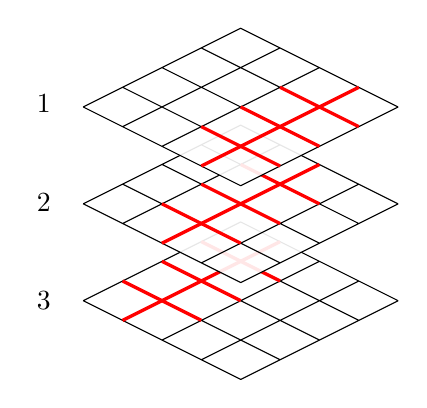
\begin{tikzpicture}[scale=0.5]

          % Nth smoothing step
          \node at (-5, 2) {$3$};
          \begin{scope}[
                  yshift=0,every node/.append style={
                  yslant=0.5,xslant=-1},yslant=0.5,xslant=-1
                  ]
              \fill[white,fill opacity=0.9] (0,0) rectangle (4,4);
              \draw[step=10mm] (0,0) grid (4,4);
              \draw[red, very thick] (1,3) -- (0,3);
              \draw[red, very thick] (1,3) -- (1,2);
              \draw[red, very thick] (1,3) -- (2,3);
              \draw[red, very thick] (1,3) -- (1,4);
              \draw[red, very thick] (2,3) -- (2,2);
              \draw[red, very thick] (2,3) -- (3,3);
              \draw[red, very thick] (2,3) -- (2,4);
              \draw[red, very thick] (3,3) -- (3,2);
              \draw[red, very thick] (3,3) -- (4,3);
              \draw[red, very thick] (3,3) -- (3,4);
          \end{scope}

          % 2nd smoothing step
          \node at (-5, 4.5) {$2$};
          \begin{scope}[
              yshift=70,every node/.append style={
              yslant=0.5,xslant=-1},yslant=0.5,xslant=-1
                          ]
              \fill[white,fill opacity=0.9] (0,0) rectangle (4,4);
              \draw[step=10mm] (0,0) grid (4,4);
              \draw[red, very thick] (1,2) -- (0,2);
              \draw[red, very thick] (1,2) -- (1,1);
              \draw[red, very thick] (1,2) -- (2,2);
              \draw[red, very thick] (1,2) -- (1,3);
              \draw[red, very thick] (2,2) -- (2,1);
              \draw[red, very thick] (2,2) -- (3,2);
              \draw[red, very thick] (2,2) -- (2,3);
              \draw[red, very thick] (3,2) -- (3,1);
              \draw[red, very thick] (3,2) -- (4,2);
              \draw[red, very thick] (3,2) -- (3,3);
          \end{scope}

          % 1st smoothing step
          \node at (-5, 7) {$1$};
          \begin{scope}[
              yshift=140,every node/.append style={
                  yslant=0.5,xslant=-1},yslant=0.5,xslant=-1
                ]
              \fill[white,fill opacity=0.9] (0,0) rectangle (4,4);
              \draw[step=10mm] (0,0) grid (4,4);
              \draw[red, very thick] (1,1) -- (0,1);
              \draw[red, very thick] (1,1) -- (1,0);
              \draw[red, very thick] (1,1) -- (2,1);
              \draw[red, very thick] (1,1) -- (1,2);
              \draw[red, very thick] (2,1) -- (2,0);
              \draw[red, very thick] (2,1) -- (3,1);
              \draw[red, very thick] (2,1) -- (2,2);
              \draw[red, very thick] (3,1) -- (3,0);
              \draw[red, very thick] (3,1) -- (4,1);
              \draw[red, very thick] (3,1) -- (3,2);

          \end{scope}
        \end{tikzpicture}

      \column{.5\textwidth}
        \centering

        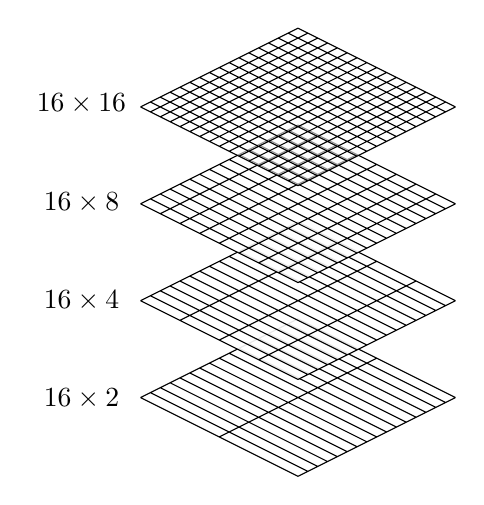
\begin{tikzpicture}[scale=0.5]

          % 16x2 Coarsest grid
          \node at (-5.5, -0.5) {$16\times2$};
          \begin{scope}[
                  yshift=-70,every node/.append style={
                  yslant=0.5,xslant=-1},yslant=0.5,xslant=-1
                  ]
              \fill[white,fill opacity=0.9] (0,0) rectangle (4,4);
              \draw[xstep=2.5mm,ystep=20mm] (0,0) grid (4,4);
          \end{scope}

          % 16x4
          \node at (-5.5, 2) {$16\times4$};
          \begin{scope}[
              yshift=0,every node/.append style={
                  yslant=0.5,xslant=-1},yslant=0.5,xslant=-1
                          ]
              \fill[white,fill opacity=.9] (0,0) rectangle (4,4);
              \draw[xstep=2.5mm,ystep=10mm] (0,0) grid (4,4);
          \end{scope}

          % 16x8
          \node at (-5.5, 4.5) {$16\times8$};
          \begin{scope}[
              yshift=70,every node/.append style={
              yslant=0.5,xslant=-1},yslant=0.5,xslant=-1
                          ]
              \fill[white,fill opacity=.9] (0,0) rectangle (4,4);
              \draw[xstep=2.5mm,ystep=5mm] (0,0) grid (4,4);
          \end{scope}

          % 16x16 Finest grid
          \node at (-5.5, 7) {$16\times16$};
          \begin{scope}[
              yshift=140,every node/.append style={
                  yslant=0.5,xslant=-1},yslant=0.5,xslant=-1
                ]
              \fill[white,fill opacity=0.6] (0,0) rectangle (4,4);
              \draw[step=2.5mm] (0,0) grid (4,4);

          \end{scope}
        \end{tikzpicture}

    \end{columns}

  \end{frame}

  \begin{frame}%
    {Analysis -- Result}
    \centering
      \includegraphics[width=.7\textwidth]{fullspace-time}
  \end{frame}

\end{document}
